\section{Literatür verisiyle yazılım uygulamaları}
\label{sec:spss-b04}

\textbf{Amaç ve veri.} \texttt{b04.csv}, \citet{cortez2008data} matematik
notlarının ampirik dağılımından geri koyarak üretilen 2.000 tekrar içerir.
Her tekrarda ilk 5 ve ilk 30 çekimin ortalaması kaydedilmiştir. Bunlar yeni
öğrenci gözlemleri değildir. Sabit tohum 2026'dır; üretim algoritması
\texttt{build\_package.py} içindedir. SPSS, hazır tekrarların dağılımını özetler.


\textbf{Ortak veri.} Doğrulanan B04 uygulamasında üç yazılım da
\nolinkurl{companion/spss/csv/b04.csv} dosyasındaki hazır tekrarları
kullanmıştır. Dosya 2.000 satır ve üç sütun içerir: \texttt{rep},
\texttt{ort5}, \texttt{ort30}. B01'in öğrenci dosyası bu uygulamada
kullanılmaz. Bu karşılaştırma Excel içe aktarmanın doğrulandığı anlamına
gelmez. Kodları \texttt{companion} klasörünü içeren paket kökünden
çalıştırın; veri sözlüğü ve hazırlık için bkz. sayfa~\pageref{sec:spss-guide}.

\subsection{IBM SPSS uygulaması}
\textbf{Başlamadan önce.} Aşağıdaki komut dosyası B04 CSV verisini
açar ve özetler. Menü yolunu kullanacaksanız önce veri açma ve tanımlama
komutlarını \texttt{EXECUTE} satırı dahil çalıştırın.

\begin{spssadimlar}
\spssadim{\texttt{b04} verisinde her satırın bir benzetim tekrarı olduğunu kontrol edin. \texttt{rep} öğrenci kimliği değil, tekrar numarasıdır.}
\spssadim{\emph{Analyze $\to$ Descriptive Statistics $\to$ Descriptives} yolunda \texttt{ort5} ve \texttt{ort30} değişkenlerini seçin.}
\spssadim{\emph{Options} altında ortalama, standart sapma, minimum ve maksimumu seçin; \emph{Continue $\to$ OK} ile özetleri alın.}
\spssadim{\emph{Graphs $\to$ Legacy Dialogs $\to$ Histogram} yolunda \texttt{ort5} seçin. \emph{Display normal curve} işaretleyip \emph{OK} seçin.}
\spssadim{Aynı histogram işlemini \texttt{ort30} için tekrarlayın. Normal eğri yalnız görsel karşılaştırmadır; normallik testi sonucu değildir.}
\end{spssadimlar}

{\raggedright
\noindent\textbf{Komutların görevi.} \texttt{DESCRIPTIVES} tekrar ortalamalarını özetler. \texttt{GRAPH /HISTOGRAM(NORMAL)} normal eğrili histogram çizer; yeni benzetim üretmez.\par}

\textbf{Uygulama kodu:} \texttt{b04}. Doğrulanan veri dosyası
\texttt{companion/spss} altındaki \texttt{csv/b04.csv} dosyasıdır.

\begin{lstlisting}[style=prismSPSS]
SET DECIMAL=DOT.
GET DATA /TYPE=TXT
 /FILE='companion/spss/csv/b04.csv'
 /ENCODING='UTF8'
 /ARRANGEMENT=DELIMITED
 /DELCASE=LINE
 /DELIMITERS="," /QUALIFIER='"'
 /FIRSTCASE=2
 /VARIABLES=rep F8.0 ort5 F20.12 ort30 F20.12.
FILTER OFF.
WEIGHT OFF.
SPLIT FILE OFF.
VARIABLE LABELS
 rep 'Benzetim tekrar numarasi'
 ort5 '5 cekimin ortalamasi'
 ort30 '30 cekimin ortalamasi'.
VARIABLE LEVEL rep (NOMINAL) ort5 ort30 (SCALE).
FORMATS ort5 ort30 (F10.6).
EXECUTE.
DESCRIPTIVES VARIABLES=ort5 ort30
 /STATISTICS=MEAN STDDEV MIN MAX.
GRAPH /HISTOGRAM(NORMAL)=ort5.
GRAPH /HISTOGRAM(NORMAL)=ort30.
\end{lstlisting}

\begin{outputguidebox}
\textbf{Paylaşılan SPSS çıktısıyla doğrulanan değerler.}
\texttt{ort5} için ortalamaların ortalaması \SPSimFiveMean, standart
sapması \SPSimFiveSD; \texttt{ort30} için sırasıyla \SPSimThirtyMean\ ve
\SPSimThirtySD\ bulunmuştur. İki dağılımın merkezi kaynak dosyanın
\SPMatMean\ ortalamasına yakındır; 30 gözlemli ortalamaların dağılımı daha
dardır. Tablodaki \emph{N}=2.000, bir örneklemin öğrenci sayısı değil,
benzetim tekrar sayısıdır. Aynı tekrar içindeki 5 ve 30 gözlemli ortalamalar
ortak çekimler içerir; bağımsız iki grup gibi test edilmez.
\end{outputguidebox}


\par\noindent\begin{minipage}{\linewidth}
\subsection{R uygulaması}
\label{sec:r-gercek-b04}

\texttt{sapply} her tekrar-ortalaması sütununu özetler; normal eğri sütunun ortalama ve standart sapmasıyla çizilir.

\begin{lstlisting}[style=prismR]
d <- read.csv("companion/spss/csv/b04.csv")
stopifnot(!anyNA(d))
print(sapply(d[c("ort5", "ort30")], function(v)
  c(n=length(v), mean=mean(v), sd=sd(v),
    min=min(v), max=max(v))))
par(mfrow=c(1, 2))
for (v in c("ort5", "ort30")) {
  x <- d[[v]]
  hist(x, breaks=seq(0, 20, by=.5),
       probability=TRUE, main=v, xlab=v,
       xlim=c(0, 20), ylim=c(0, .6))
  curve(dnorm(x, mean(d[[v]]), sd(d[[v]])),
        add=TRUE, col="blue")
}
par(mfrow=c(1, 1))
\end{lstlisting}

\textbf{Çıktıyı okuma.} Paylaşılan R çıktısı 2.000 satır ve üç sütun
gösterir; her sütunda eksik değer sayısı sıfırdır. \texttt{n},
\texttt{mean}, \texttt{sd}, \texttt{min} ve \texttt{max} satırları
ortak tabloda özetlenmiştir. Buradaki \texttt{n}, tekrar sayısıdır.
\end{minipage}\par

\par\noindent\begin{minipage}{\linewidth}
\subsection{Python uygulaması}
\label{sec:python-b04}

\texttt{density=True} histogramı yoğunluk ölçeğine getirir; normal eğri aynı sütunun özetleriyle çizilir.

\begin{lstlisting}[style=prismPythonApp]
import pandas as pd
import numpy as np
from scipy import stats
import matplotlib.pyplot as plt

d = pd.read_csv("companion/spss/csv/b04.csv")
assert not d.isna().any().any()
print(d[["ort5", "ort30"]].agg(
    ["count", "mean", "std", "min", "max"]))
fig, axes = plt.subplots(1, 2)
for ax, v in zip(axes, ["ort5", "ort30"]):
    x = d[v]
    ax.hist(x, bins=np.arange(0, 20.5, .5), density=True)
    grid = np.linspace(0, 20, 1000)
    ax.plot(grid, stats.norm.pdf(grid, x.mean(), x.std()))
    ax.set_title(v)
    ax.set_xlim(0, 20); ax.set_ylim(0, .6)
plt.tight_layout(); plt.show()
\end{lstlisting}

\textbf{Çıktıyı okuma.} Paylaşılan Python çıktısında da 2.000 satır,
üç sütun ve her sütunda sıfır eksik değer vardır. \texttt{count}, R'deki
\texttt{n}; \texttt{std} ise \texttt{sd} satırına karşılık gelir.
Bu uygulama bir hipotez testi veya $p$ değeri üretmez.
\end{minipage}\par

\subsection{Sonuçların karşılaştırılması ve ortak rapor}
12 Eylül 2026'da paylaşılan SPSS tablosu ve histogramları, R ve Python
metin çıktıları ve grafikleriyle karşılaştırılmıştır. İki değişkene ait
10 betimsel değer R ve Python'da gösterilen 11 ondalık basamakta
eşleşmiş; proje CSV'sinden yapılan hesaplar ve SPSS'in gösterdiği
yuvarlama hassasiyetiyle de uyum sağlanmıştır. Aşağıdaki tablo bu
çıktıların kitap düzenine uyarlanmış özetidir; ekran görüntüsü değildir.

\begin{table}[H]
\centering
\caption{B04 tekrar ortalamalarının doğrulanmış betimsel özetleri}
\label{tab:b04-dogrulanmis-betimsel}
\begin{tabular}{@{}lrr@{}}
\toprule
Ölçü & $n=5$ & $n=30$ \\
\midrule
Geçerli tekrar sayısı & 2.000 & 2.000 \\
Ortalamaların ortalaması & 10,367800 & 10,419050 \\
Ortalamaların std. sapması & 2,078856 & 0,844512 \\
En küçük ortalama & 2,800000 & 7,366667 \\
En büyük ortalama & 16,200000 & 13,000000 \\
\bottomrule
\end{tabular}
\par\smallskip
{\footnotesize Ondalıklı değerler altı basamağa yuvarlanmıştır.
Standart sapmalar 2.000 tekrar ortalaması üzerinden, paydada 1.999
kullanılarak hesaplanmıştır. Sütun başlıklarındaki $n$, her ortalamanın
kaç çekimden hesaplandığını belirtir.\par}
\end{table}

\begin{figure}[H]
\centering
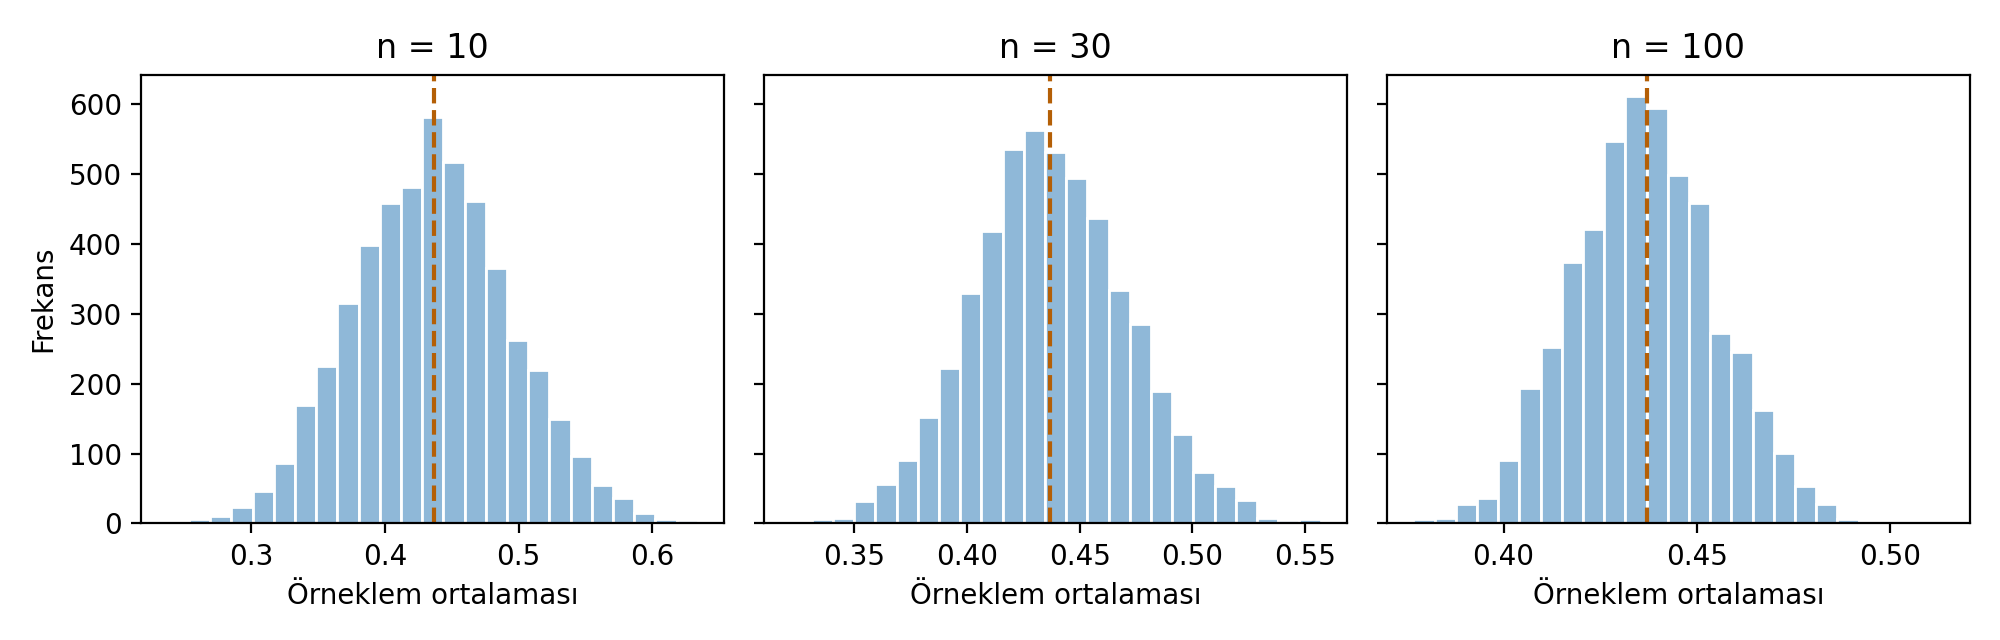
\includegraphics[width=\linewidth]{companion/outputs/figures/chapter04_sampling_means.png}
\caption{B04 için paylaşılan Python histogramları ve normal eğriler.
Sol panel 5, sağ panel 30 çekimin ortalamalarını gösterir;
yatay ve düşey ölçekler ortaktır.}
\label{fig:b04-dogrulanmis-grafikler}
\end{figure}

\Needspace{17\baselineskip}
\begin{outputguidebox}
Tablo~\ref{tab:b04-dogrulanmis-betimsel} ve
Şekil~\ref{fig:b04-dogrulanmis-grafikler}, 30 çekimlik ortalamaların
5 çekimlik ortalamalara göre daha dar dağıldığını gösterir. Buradaki
standart sapma, bireysel öğrenci notlarının değil tekrar ortalamalarının
yayılımıdır. 2.000 tekrar ile örneklem büyüklükleri 5 ve 30 karıştırılmaz.

Paylaşılan SPSS histogramları frekans, R ve Python histogramları
yoğunluk ölçeğindedir. R ve Python'da sınıf genişliği 0,5 ve yatay
aralık 0--20 olsa da sınıf sınırındaki değerlerin yerleştirilme kuralları
farklı olduğundan sütun yükseklikleri birebir eşleşmez. Normal eğriler
görsel karşılaştırma içindir; normalliği kanıtlamaz.

Hazır tekrarlar her ortamda aynıdır; yeniden rastgele çekim
yapılmadığından yazılımlar arasında tohum eşitlemek gerekmez. Hesaplama
uyumu, kaynak öğrenci verisinin daha geniş bir evreni temsil ettiğini
göstermez. Aynı satırdaki iki ortalama ortak çekimler içerir.
\end{outputguidebox}

\textbf{Raporlama örneği (doğrulanmış çıktılarla).}
``Ampirik not dağılımından geri koyarak üretilen 2.000 tekrarda,
5 çekimlik ortalamaların ortalaması 10,367800 ve standart sapması
2,078856; 30 çekimlik ortalamaların ortalaması 10,419050 ve standart
sapması 0,844512 bulunmuştur. Ortak ölçekli histogramlarda 30 çekimlik
ortalamalar daha dar bir dağılım göstermiştir. Sonuçlar yeni öğrenci
gözlemleri değil benzetim çıktılarıdır; iki sütun bağımsız gruplar
olarak test edilmemiştir.''


\textbf{Görev.} İki histogramı aynı yatay ölçekle karşılaştırın. Tek bir
öğrencinin not dağılımı ile örneklem ortalamasının dağılımını ayıran bir
cümle yazın. Geri koyarak çekim nedeniyle burada sonlu evren düzeltmesi
uygulanmadığını açıklayın.